
\chapter{Аналитическая часть}

	
	\section{Описание объектов сцены}
	
	Сцена должна состоять из наблюдателя (камеры), плоскости пола, двух людей, источника направленного света и робота Ф-2.
	Модель робота Ф-2 должен состоять из нескольких частей тела: головы, туловища, рук. Голова робота должна быть представлена в виде параллелепипеда, а руки и туловище --- в виде цилиндров.
	Модели людей также должны состоять из головы --- сферы --- а также туловища и рук --- цилиндров.
	Плоскость пола --– это некая ограничивающая плоскость. Предполагается, что под ней не расположено никаких объектов.
	
	Анимация робота должна состоять из следующей последовательности действий.
	
	1) Робот должен повернуть голову в сторону одного человека, затем в сторону другого. 
	
	2) Робот должен помахать руками первому человеку.
	
	3) Робот должен приблизиться ко второму человеку и протянуть ему руку.
	
	\section{Анализ и выбор формы представления трехмерных моделей}
	
	Отображением формы и размеров объектов являются модели. 
	Обычно используются следующие три способа описания моделей.
	
	1.	Каркасная (проволочная) модель --- одна из простейших форм задания модели, в ней хранится информация только о вершинах и ребрах объекта. Недостаток данной формы состоит в том, что модель не всегда точно передает представление о форме объекта.
	
	2.	Поверхностная модель.
	Такой тип модели часто используется в компьютерной графике. Поверхности могут быть заданы разными способами: либо аналитически, либо с использованием полигональной аппроксимации. Недостаток данной формы состоит в том, что она не нест информации о том, с какой стороны расположен материал.
	
	3.	Объемная (твердотельная) модель.
	Данная форма отличается от поверхностной тем, что содержит информацию о материале. Это делается с помощью указания направления внутренней нормали. 
	
	\textbf{Вывод:} для решения данной задачи имеет смысл использовать поверхностные модели, так как каркасные модели могут привести к неправильному восприятию формы, а объемные модели повлекут излишние затраты памяти.
	
	\section{Анализ способа представления поверхностных моделей}
	
	Также необходимо определить каким образом будут заданы поверхностные модели. Существуют два основных способа:
	 
	\textit{Аналитическй способ}. Поверхность модели описывается функцией. Например, поверхность сферы имеет вид $x^2 + y^2 + z^2 = R^2.$
	Преимущества аналитического способа задания поверхностных моделей.
	
	1) Минимальные затраты памяти.
	
	2) Быстрое выполнение операций переноса, вращения, масштабирования.
	
	3) Поверхность задаётся с абсолютной точностью, а не аппроксимируется.
	
	Недостатки аналитического способа задания поверхностных моделей.
	
	1) Задать сложную модель аналитически может быть практически невозможно.
	
	2) Скорость вычислений зависит от сложности подобранной функции.
	
	3) Проблемы при наложении текстур.
	
	\textit{Аппроксимация полигональной сеткой}. Поверхность модели описывается набором многоугольников (как правило, используются треугольники)
	
	Преимущества подхода на основе аппроксимации полигональной сеткой:
	
	1) Можно достаточно точно передать поверхность любого объекта реального мира.
	
	2) Преобразование всех моделей выполняется одинаково.
	
	3) Добавление новой модели не требует написания кода.
	
	4) Большинство алгоритмов удаления невидимых линий используют данное представление.
	
	5) Информации, содержащейся в данном представлении достаточно для необычных преобразований модели (например, для разделения модели на несколько).
	
	Недостатки подхода на основе аппроксимации полигональной сеткой.
	
	1) Большие затраты памяти.
	
	2) Скорость вычислений зависит от количества вершин у модели.
	
	3) Модель может быть передана некачественно.
		
	\textbf{Вывод:} в поставленной задаче нет необходимости в сложных поверхностях, так что наиболее подходящим булет аналитический способ представления моделей. Ключевыми для принятия этого решения оказались экономия памяти и быстрота преобразований в пространстве, достигаемые аналитическим представлением моделей. Самым ярким примером будет сравнение сложности представления сферы обоими способами.

	\section{Анализ и выбор алгоритма удаления невидимых линий и поверхностей}
	
	Перед выбором алгоритма удаления невидимых рёбер и поверхностей  необходимо отметить, что для эффективного решения поставленной задачи алгоритм должен удовлетворять следующим требованиям: быстродействие, малое потребление памяти и возможность использовать выбранный формат представления модели (аналитический).
	

\subsection{Алгоритм, использующий Z-буфер}

Суть данного алгоритма – это использование двух буферов: буфера кадра, в котором хранятся атрибуты каждого пикселя, и Z-буфера, в котором хранятся информация о координате Z для каждого пикселя.

Первоначально в z-буфере находятся минимально возможные значения Z, а в буфере кадра располагаются пиксели, описывающие фон. Каждый многоугольник преобразуется в растровую форму и записывается в буфер кадра.

В процессе подсчета глубины нового пикселя, он сравнивается с тем значением, которое уже лежит в z-буфере. Если новый пиксель расположен ближе к наблюдателю, чем предыдущий, то он заносится в буфер кадра и происходит корректировка z-буфера.
Для решения задачи вычисления глубины Z каждый многоугольник описывается уравнением $ax+by+cz+d=0$. При c=0 многоугольник для наблюдателя вырождается в линию.
 
Для некоторой сканирующей строки $y=const$, поэтому имеется возможность рекуррентно высчитывать $z'$ для каждого $x'=x+dx$.

Преимущества алгоритма, использующего Z-буфер.

1)	Простота реализации алгоритма.

2)  Оценка трудоемкости линейна.

Недостатки алгоритма, использующего Z-буфер.

1) Большие затраты памяти.

2) Сложное добавление функционала освещения и прозрачности.

3) Требует придставления модели в виде полигональной сетки.

\textbf{Вывод}: Алгоритм не удовлетворяет ключевым требованиям.


\subsection{Алгоритм художника}

У вышеуказанного алгоритма “говорящее” название, потому что его работа схожа с рисованием картины художником. Как художники рисуют картину: предварительно наносятся на рисунок более далёкие объекты и только позднее наносятся близкие к наблюдателю объекты. При реализации данного алгоритма используют сортировку (по глубине). Цель сортировки в том, что все грани сортируются таким образом, чтобы отрисовка наиболее близких граней была произведена в конце, то есть сначала рисуются самые далёкие грани и только потом – ближние грани. Рассмотрим положительные стороны и недостатки данного алгоритма.
	
Преимущества алгоритма художника.

1.	Линейно-логарифмическая оценка трудоемкости.

2.	Малое использование памяти. 

Недостатки алгоритма художника.

1.	Сложность реализации пересекающихся граней.

2.	Результирующая картина не обладает достаточной реалистичностью.

3.	Многократное перекрашивание одного и того же пиксела.

4.	Требует представления модели в виде полигональной сетки.

\textbf{Вывод}: Алгоритм не удовлетворят ключевым требованиям.

\subsection{Алгоритм обратной трассировки лучей}

Суть алгоритма обратной трассировки лучей (в оригинале --- Ray Tracing) состоит в том, что наблюдатель видит объект с помощью испускаемого света, который согласно законам оптики доходит до наблюдателя некоторым путем. Отслеживать пути лучей от источника к наблюдателю неэффективно с точки зрения вычислений, поэтому наилучшим способом будет отслеживание путей в обратном направлении, то есть от наблюдателя к объекту.

\begin{figure}[h]
	\centering
	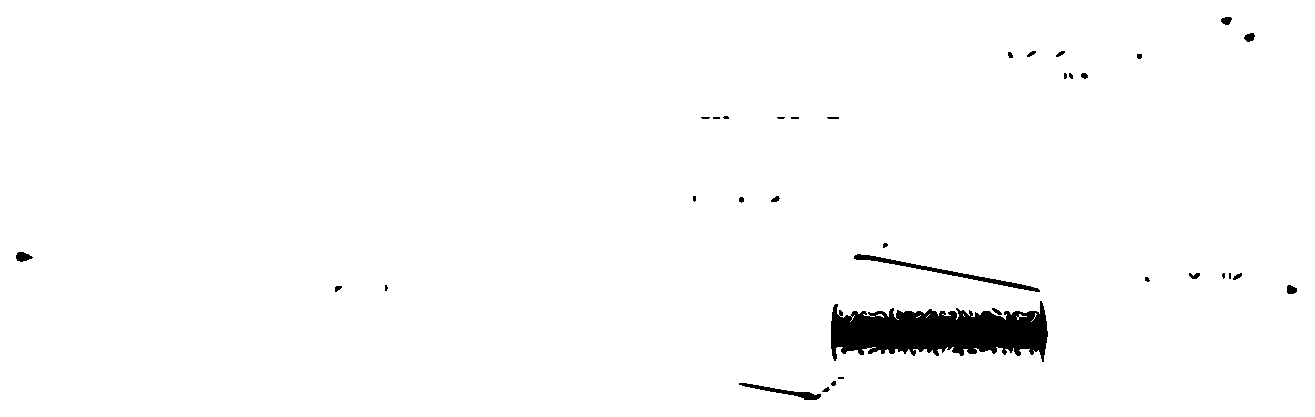
\includegraphics[width=0.9\linewidth]{images/screenshot003}
	\caption{Иллюстрация обратной трассировки лучей}
	
	\label{fig:screenshot003}
\end{figure}
	
Преимущества алгоритма обратной трассировки лучей.

1.  Высокая реалистичность синтезируемого изображения.

2.	Может работать с поверхностями в аналитической форме.

3.	Могут быть применены параллельные вычисления.

Основной недостаток алгоритма обратной трассировки лучей --- низкая производительность реализаций алгоритма.
	
\textbf{Вывод}: данный алгоритм в первую очередь используется для получения реалистичного изображения, что сказывается на его быстродействии, однако алгоритм может быть более эффективным, если его адаптировать к решаемой задаче.

\subsection{Алгоритм Робертса}

Алгоритм Робертса имеет свои особенности, он работает в объектном пространстве, но при этом он рисует сцену только с выпуклыми телами --– это необходимое условие для валидной отработки алгоритма.

Данный алгоритм имеет 3 этапа и один предварительный:

Предварительный этап --- подготовка исходных данных. Необходимо для каждого тела сформировать матрицу тела размерностью 4xN, где N --– количество граней тела.

1.	Удаление рёбер, экранируемых самим телом.

Определим вектор $E = (0, 0, -1, 0)$ как вектор взгляда наблюдателя. Чтобы понять, какие грани отрисовать нужно, а какие --– не нужно, нужно умножить вектор взгляда на матрицу тела. Отрицательные величину результирующей матрицы свидетельствуют о невидимых гранях.

2.	Удаление рёбер, экранируемых другими телами.

На этом шаге используется луч, который “испускается” от точки наблюдателя до точки на ребре. Если луч пересекает какую-либо грань, значит точка невидима.

3.	Удаление линий пересечения тел, экранируемых самими телами и другими телами, связанными отношением протыкания.

Если тела связаны отношением взаимного протыкания, то будут образовываться новые рёбра, и также требуется определить их видимость. На данном этапе на рассматриваются рёбра, которые соединяют невидимые точки, так как в этом нет смысла. И в результате новые рёбра проверяются на экранирование другими телами сцены и самими телами.
	
Преимущества алгоритма Робертса.

1.	Высокая точность вычислений.

2.	Алгоритм используется в объектном пространстве.
	
Недостатки алгоритма Робертса.

1.	Квадратичная сложность алгоритма, в зависимости от количества объектов.

2.	Объекты сцены обязательно должны быть выпуклыми многоугогранниками.

3.	Высокая сложность реализации алгоритма.

\textbf{Вывод}: алгоритм не удовлетворят ключевым требованиям.

\subsection {Алгоритм марширования лучей}

 В алгоритме марширования лучей (в оригинале --- Ray Marching) вся сцена определяется в терминах функции расстояния со знаком. Чтобы найти пересечение между лучом обзора и сценой, постепенно перемещается точка от камеры вдоль направления луча. На каждом шаге, при помощи функции расстояния определяется, вошла ли точка в какое-либо тело. [5]

В целях повышения производительности реализаций алгоритма, расстояние, на которое смещается точка не является фиксированно-маленьким, оно вычисляется каждую итерацию, как максимально допустимое, не приводящее к прохождению луча сквозь поверхность.

\begin{figure}[h]
	\centering
	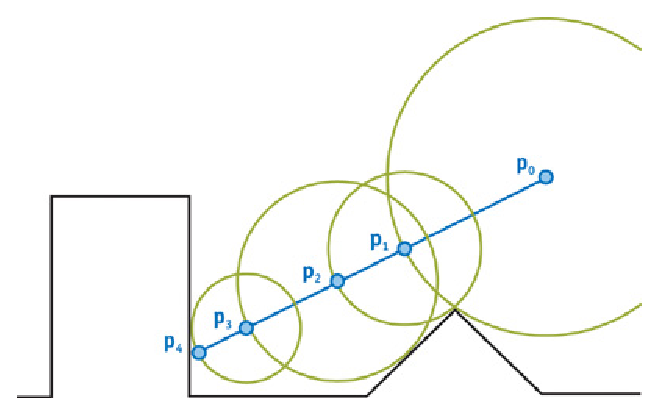
\includegraphics[width=0.7\linewidth]{images/spheretrace}
	\caption{Иллюстрация "маршировки" лучей}
	\label{fig:spheretrace}
\end{figure}

Преимущества алгоритма марширования лучей:

1. Алгоритм использует модели в аналитической форме.

2. Не требователен по памяти.

3. Позволяет визуализировать необычные поверхности, например, трёхмерные фракталы.

4. Изображение получается идеально гладким.

5. Могут быть применены параллельные вычисления.

Недостатки алгоритма марширования лучей.

1.	Алгоритм очень сильно теряет в производительности с ростом количества объектов на сцене.

2.	Все недостатки аналитического представления поверхности.

\textbf{Вывод}: алгоритм может быть использован для решения задачи, однако его реализация будет неэффективной по времени.

\textbf{Вывод из анализа алгоритмов удаления невидимых линий и поверхностей:}
из всех перечисленных алгоритмов только два могут быть применены к аналитически заданным поверхностям. Из этих алгоритмов выбор пал на обратную трассировку лучей, так как она окажется более быстродейственной, при оптимизации под нашу задачу.
	
\section{Анализ и выбор модели освещения}

\subsection*{Модель Ламберта}
	
	 Модель Ламберта включает только идеальное диффузное освещение, то есть свет при попадании на поверхность рассеивается равномерно во все стороны. При такой модели освещения учитывается только ориентация поверхности (N) и направление источника света (L) (рис. ~\ref{fig:screenshot001}):	
\begin{equation}
	I = I_{p} \cdot k_{p} + \dfrac{I_{u} \cdot k_{d} \cdot \cos\theta}{d + K}
\end{equation}
где 
	$I_{p}$ --- интенсивность рассеянного света;
	
	$k_{p}$ --- коэффициент диффузного отражения рассеянного света
	
	$I_{u}$ --- интенсивность точечного источника света
	
	$k_{d}$ --- коэффициент диффузного отражения
	
	$\theta$ --- угол между нормалью к поверхности и направление света
	
	$d$ --- расстояние от центра проекции до объекта
	
	$K$ --- произвольная константа

\newpage
\begin{figure}[h]
	\centering{}
	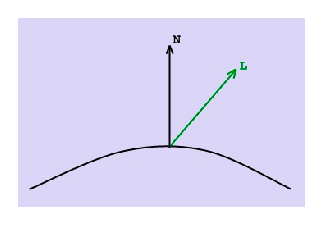
\includegraphics[width=0.7\linewidth]{screenshot001}
	\caption{Иллюстрация модели Ламберта}
	\label{fig:screenshot001}
\end{figure}

Эта модель является одной из самых простых моделей освещения и очень часто используется в комбинации с другими моделями. Она может быть удобна для анализа свойств других моделей, за счет того, что ее легко выделить из любой модели и анализировать оставшиеся составляющие.

\subsection* {Модель Фонга}

 Модель Фонга (простая модель освещения) представляет собой комбинацию диффузной и зеркальной составляющих. Работает модель таким образом, что кроме равномерного освещения на материале могут появляться блики. Местонахождение блика на объекте определяется из закона равенства углов падения и отражения. Чем ближе наблюдатель к углам отражения, тем выше яркость соответствующей точки: 
\begin{equation}
	I = I_{p}\cdot k_{p} + \dfrac{I_{u}}{d + K} \cdot(k_{d}\cdot\cos(\theta) + k_{3}\cdot cos^{n}(\alpha)),
\end{equation}
где
	$I_{p}$ --- интенсивность рассеяного света
	
	$k_{p}$ --- коэффициент диффузного отражения рассеяного света
	
	$I_{u}$ --- интенсивность точечного источника света
	
	$k_{d}$ --- коэффициент диффузного отражения
	
	$\theta$ --- угол между нормалью к поверхности (n) и направлением света (L)
	
	$d$ --- расстояние от центра проекции до объекта
	
	$K$ --- произвольная константа
	
	$k_{3}$ --- коэффициент зеркального отражения
	
	$\alpha$ --- угол между вектором наблюдения (S) и отраженным лучом (R)
	
	$n$ --- степень, аппроксимирующая пространственное распределение зеркально отраженного света


\begin{figure}[h]
	\centering
	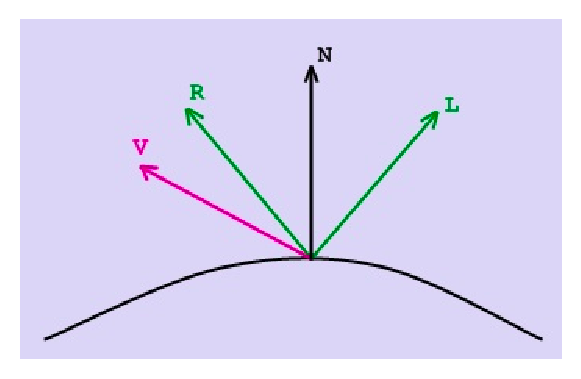
\includegraphics[width=0.7\linewidth]{images/screenshot002}
	\caption{Иллюстрация модели Фонга}
	\label{fig:screenshot002}
\end{figure}

Падающий и отраженный лучи лежат в одной плоскости с нормалью к отражающей поверхности в точке падения (рис. ~\ref{fig:screenshot002}). Нормаль делит угол между лучами на две равные части. L --– направление источника света, R --– направление отраженного луча, V --– направление на наблюдателя.

\subsection* {Глобальная модель освещения}

Глобальная модель будет содержать в себе те же составляющие, что и простая модель освещения, но ещё учитывать интенсивность рассеянного освещения, зеркально отраженный свет от других поверхностей и пропускание света прозрачными поверхностями.

\begin{equation}
	I = I_{p} \cdot k_{p} + k_{d} \cdot \sum_{j} I_{uj} \cdot \cos\theta_{j} + k_{s} \cdot \sum_{j} I_{u} \cdot cos^{n} \alpha_{j} + k_{s} \cdot I_{s} + k_{t} \cdot I_{t}
\end{equation}

где

	$I_{p}$ --- интенсивность рассеяного света
	
	$k_{p}$ --- коэффициент диффузного отражения рассеяного света
	
	$I_{u}$ --- интенсивность точечного источника света
	
	$k_{d}$ --- коэффициент диффузного отражения
	
	$\theta$ --- угол между нормалью (n) к поверхности и направлением света (v)
	
	$d$ --- расстояние от центра проекции до объекта
	
	$K$ --- произвольная константа
	
	$k_{s}$ --- коэффициент зеркального отражения
	
	$\alpha$ --- угол между вектором наблюдения (S) и отраженным лучом (r)
	
	$n$ --- степень, аппроксимирующая пространственное распределение зеркально отраженного света
	
	$k_{t}$ --- коэффициент пропускания
	
	$I_{t}$ --- интенсивность света, падающего в точку по направлению \textbf{p}
	
	$I_{s}$ --- интенсивность зеркально отраженного света

	\textbf{Вывод:} глобальная модель освещения является слишком затратной по времени, а модель Ламберта недостаточно хорошо передаёт геометрию сцены, поэтому была выбрана модель освещения Фонга.
	
	\section{Анализ и выбор способа анимирования объектов сцены}
	
	\subsection*{Метод ключевых кадров}
	
	При данном подходе анимационная последовательность задается в терминах ключей. Каждый ключ представляет позицию и ориентацию, которые должен занять заданный объект в определенный момент времени. Позиция и ориентация объекта на протяжении анимационной последовательности вычисляется на основе этих ключей~[7].
	
	
	\subsection*{Метод кривых движения}
	
	При данном подходе анимационная последовательность задается с помощью кривых движения. Кривые движения --- это представление перемещения или трансформации объекта в виде графиков для каждой из его координат XYZ~[7].
	
	
	\textbf{Вывод}: отличие методов анимирования по производительности несущественно, поэтому выбран метод ключевых кадров как более простой в реализации и использовании.